\section{訂閱功能}

\begin{frame}{活動數據分析}
\only<1-10>{
\begin{itemize}
\item 照著功率/心率/速度/坡度/溫度等數據的高低畫出的地圖\pause
\item 功率區間/心率區間/區段配速\\\pause
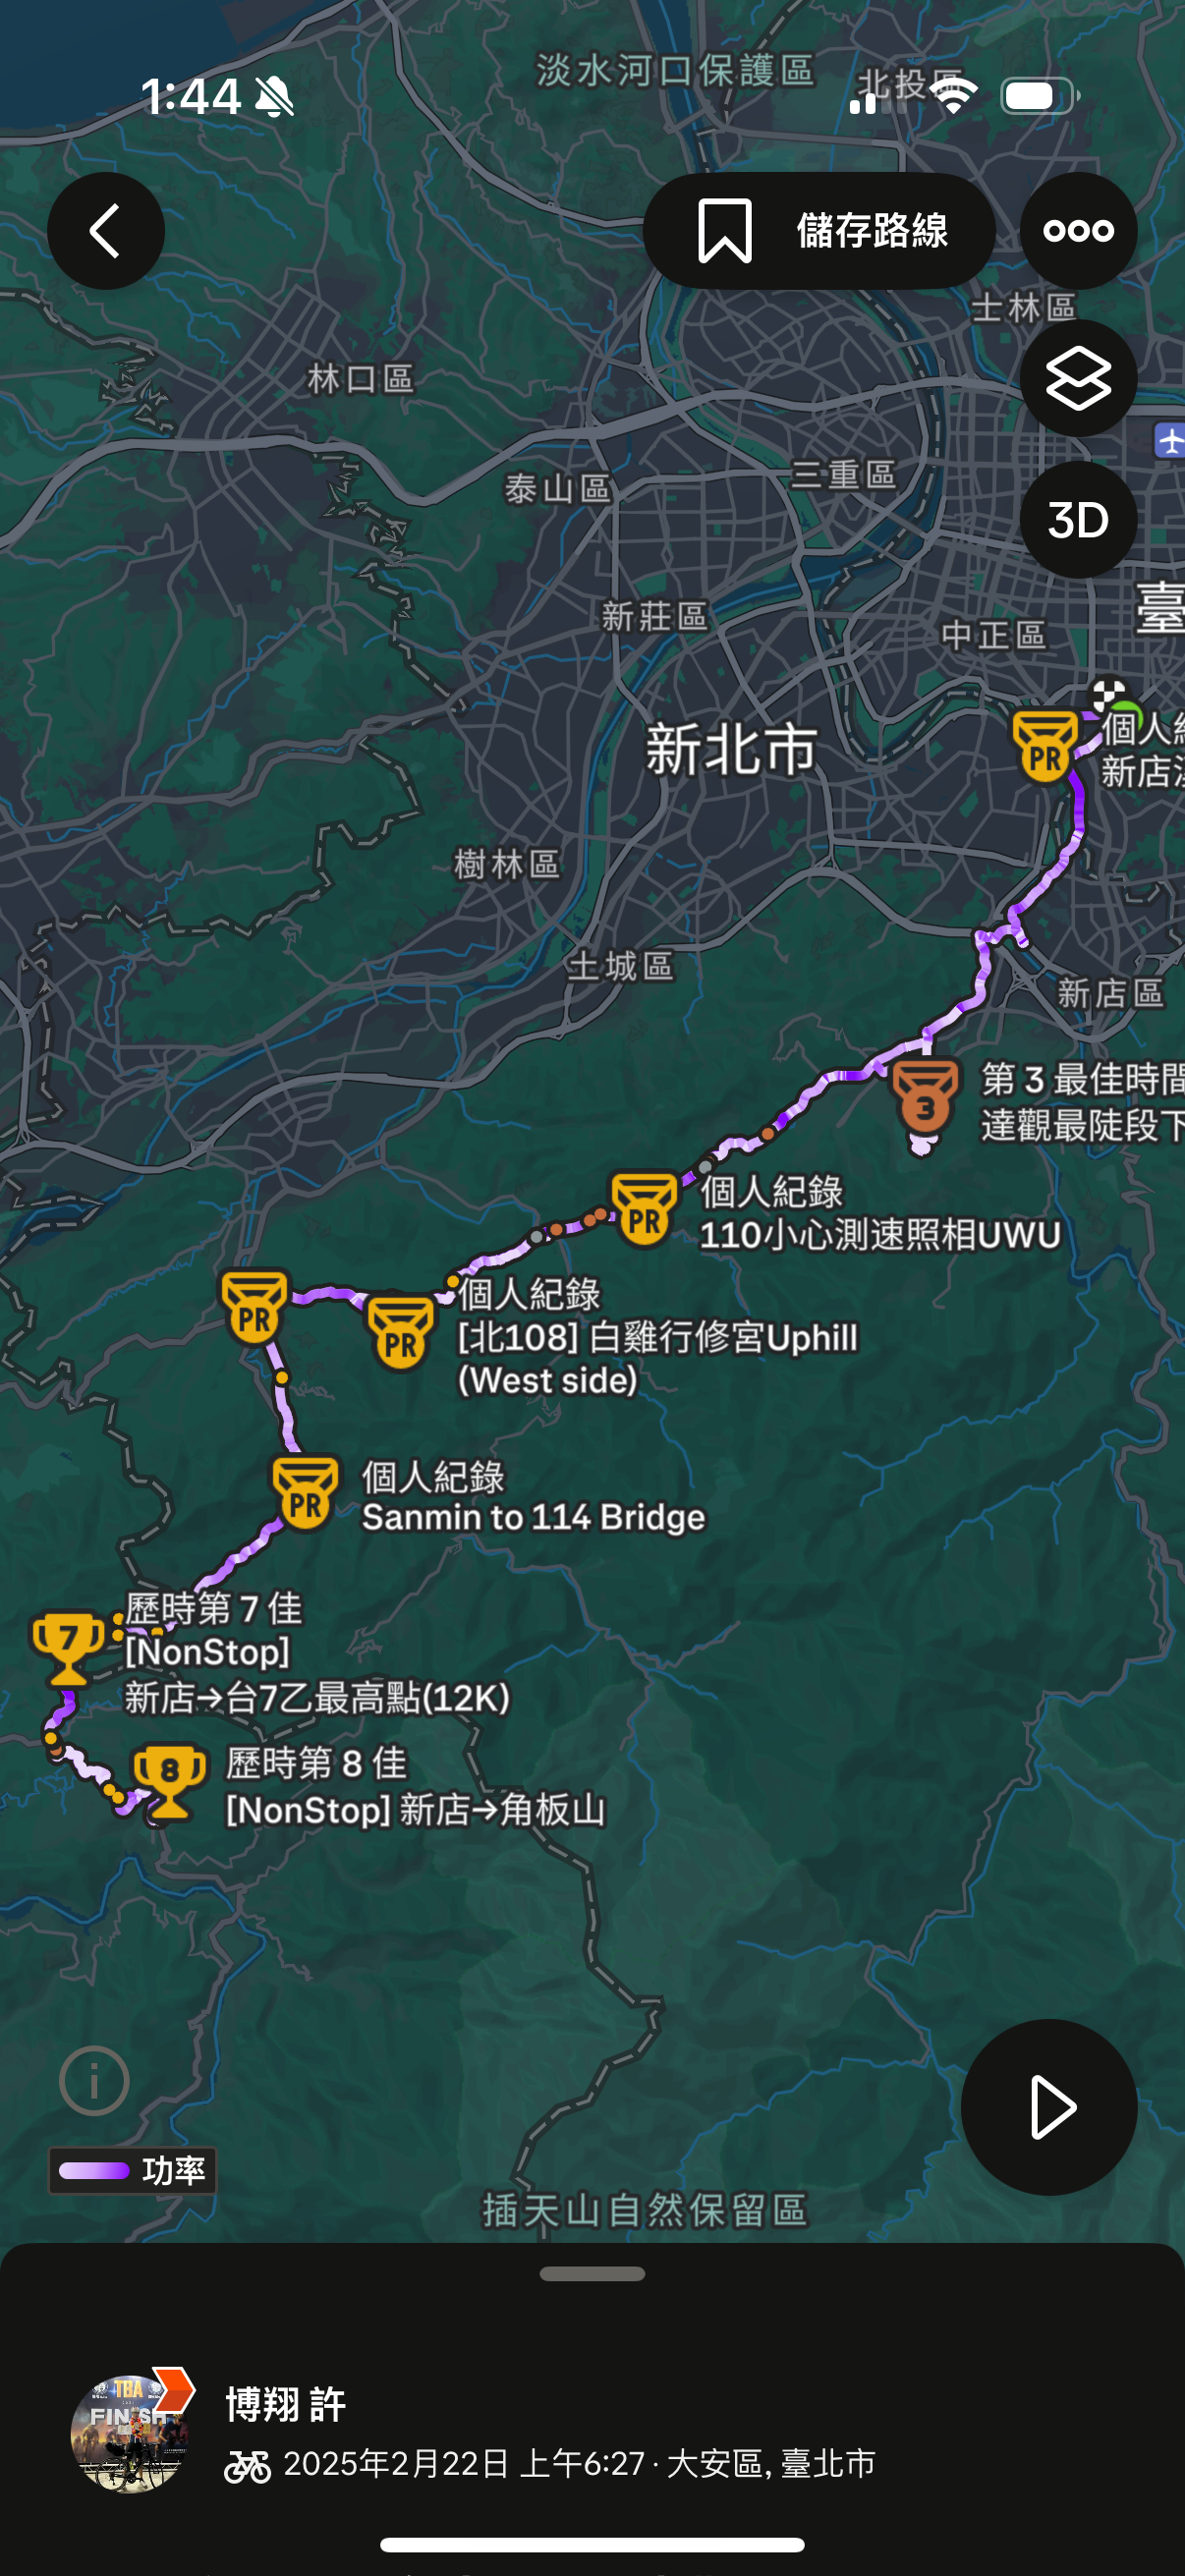
\includegraphics[height=5cm]{subscribe1.png}\pause
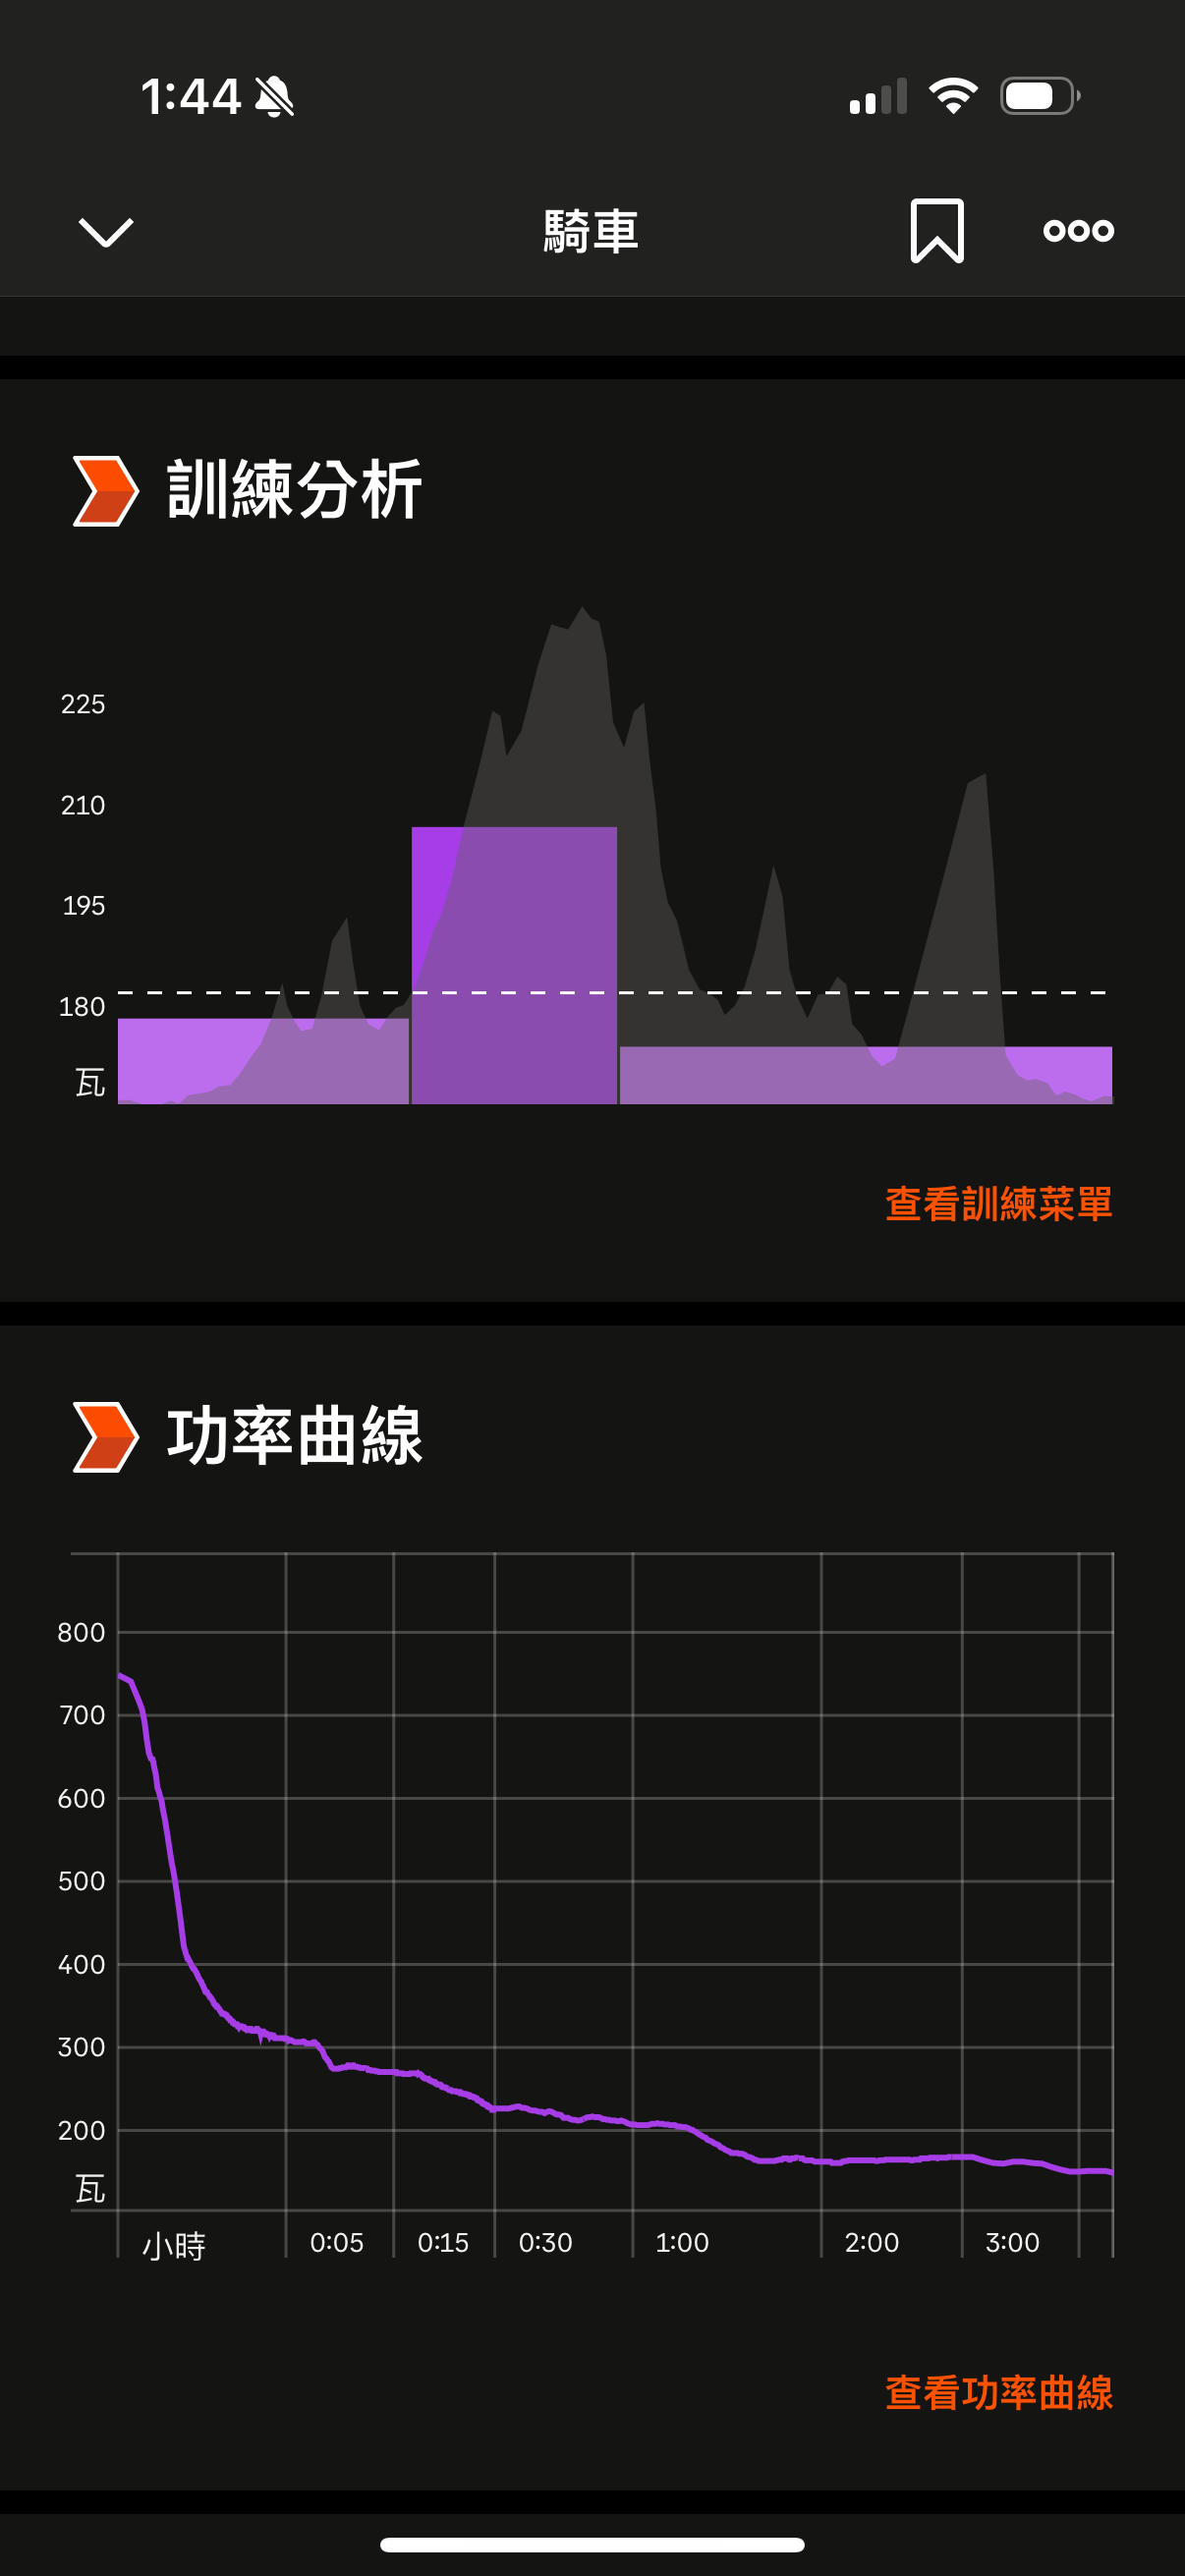
\includegraphics[height=5cm]{subscribe2.png}\pause
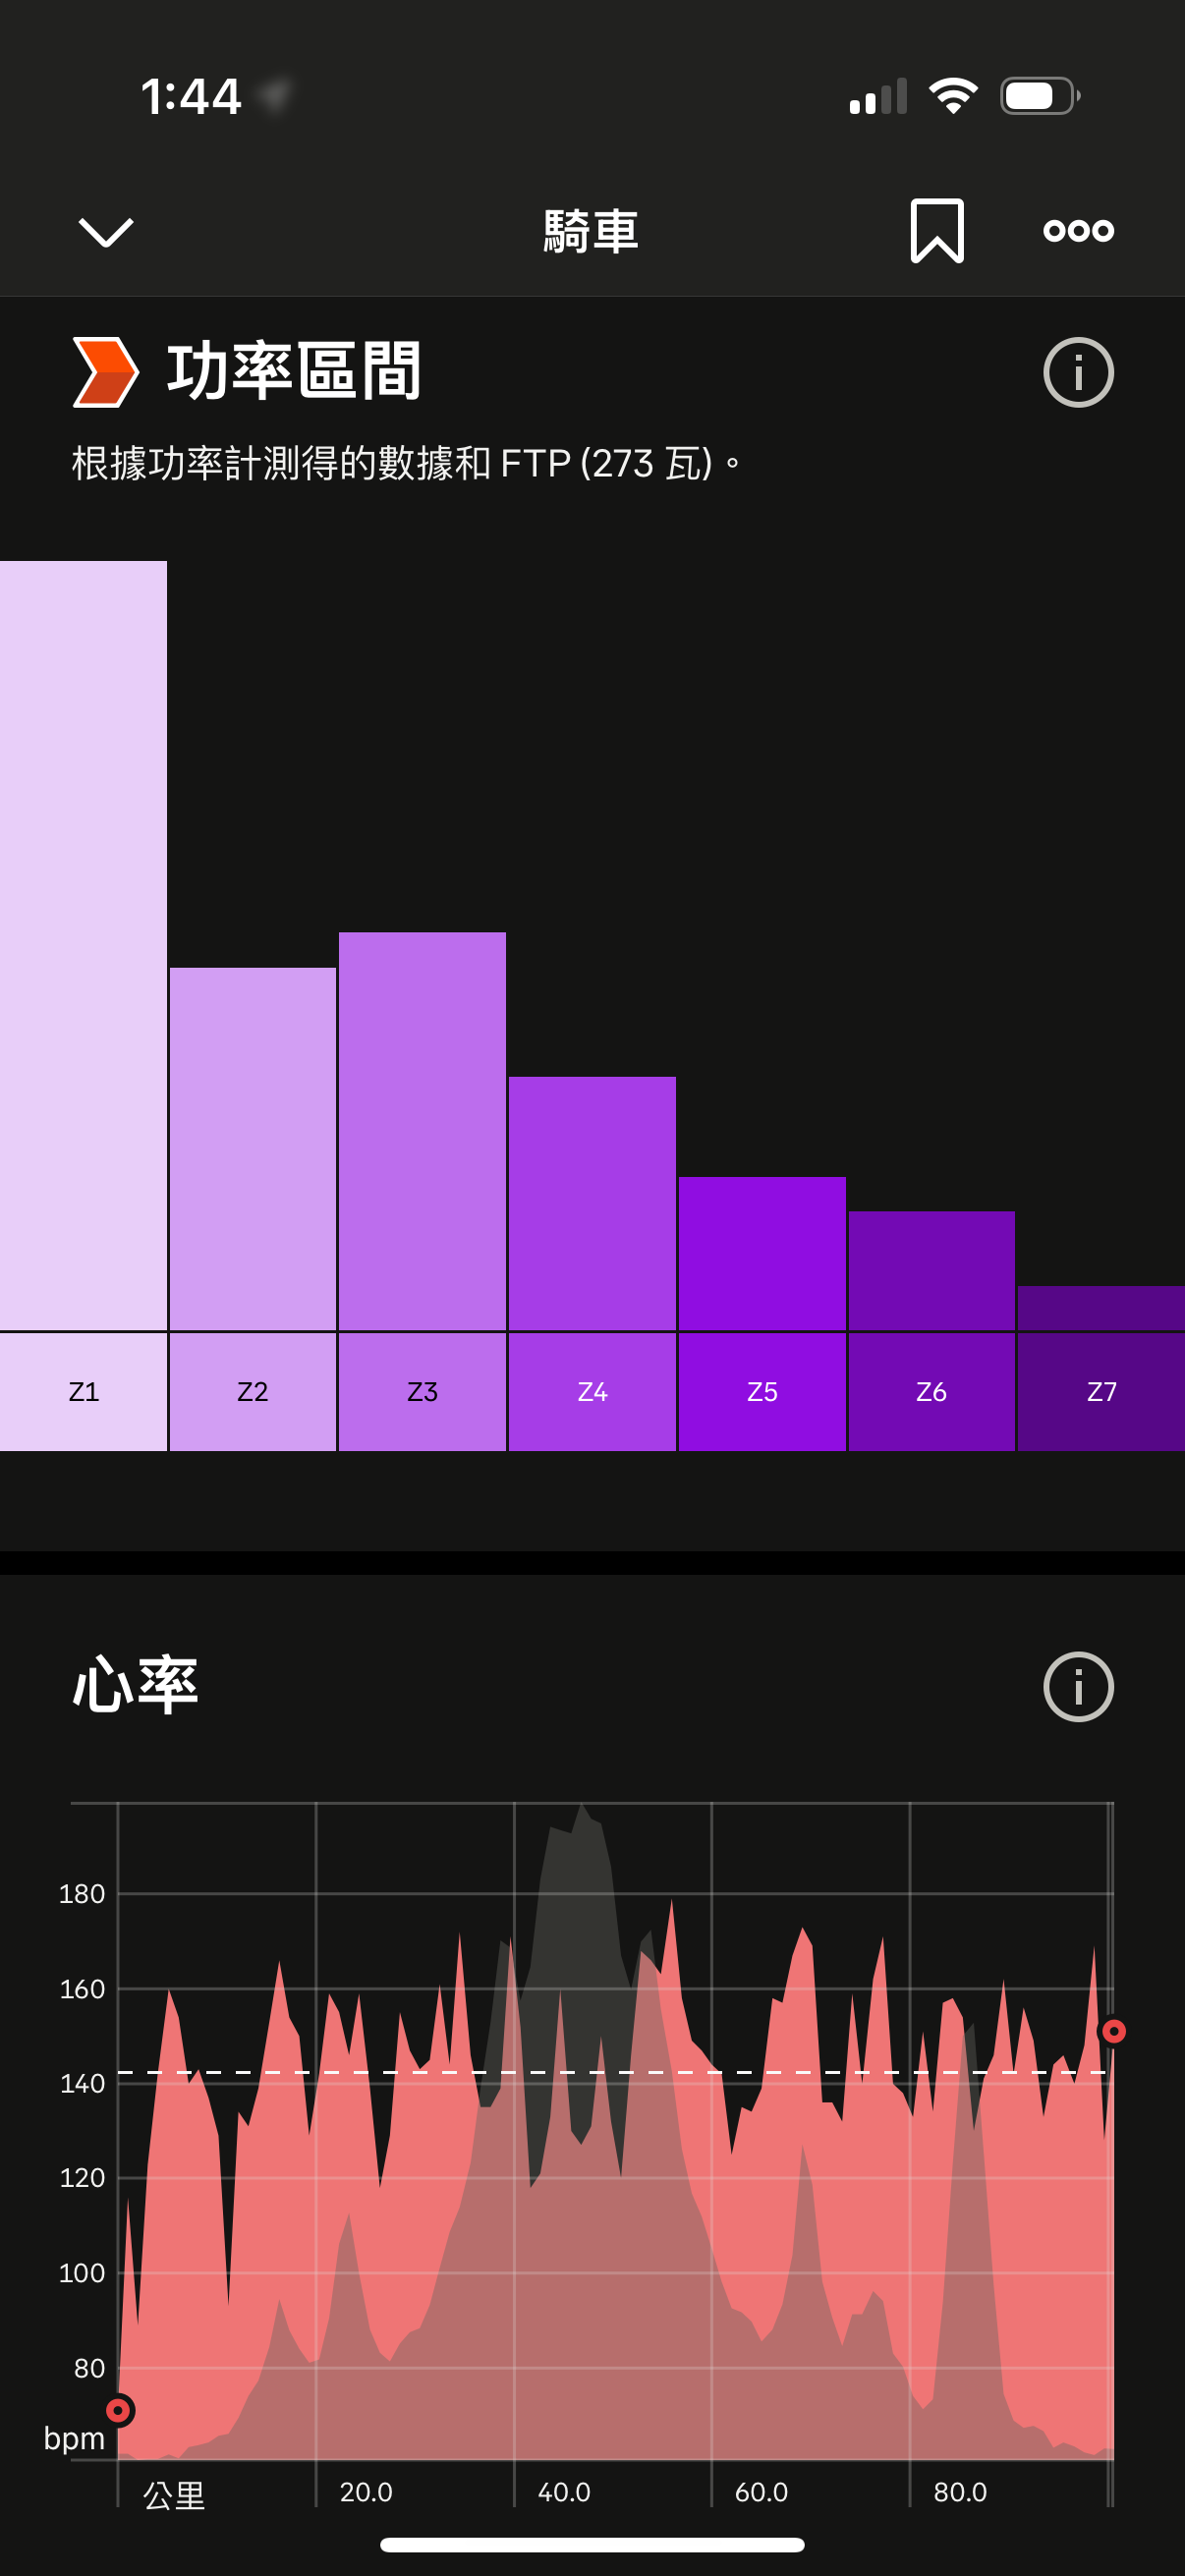
\includegraphics[height=5cm]{subscribe3.png}\pause
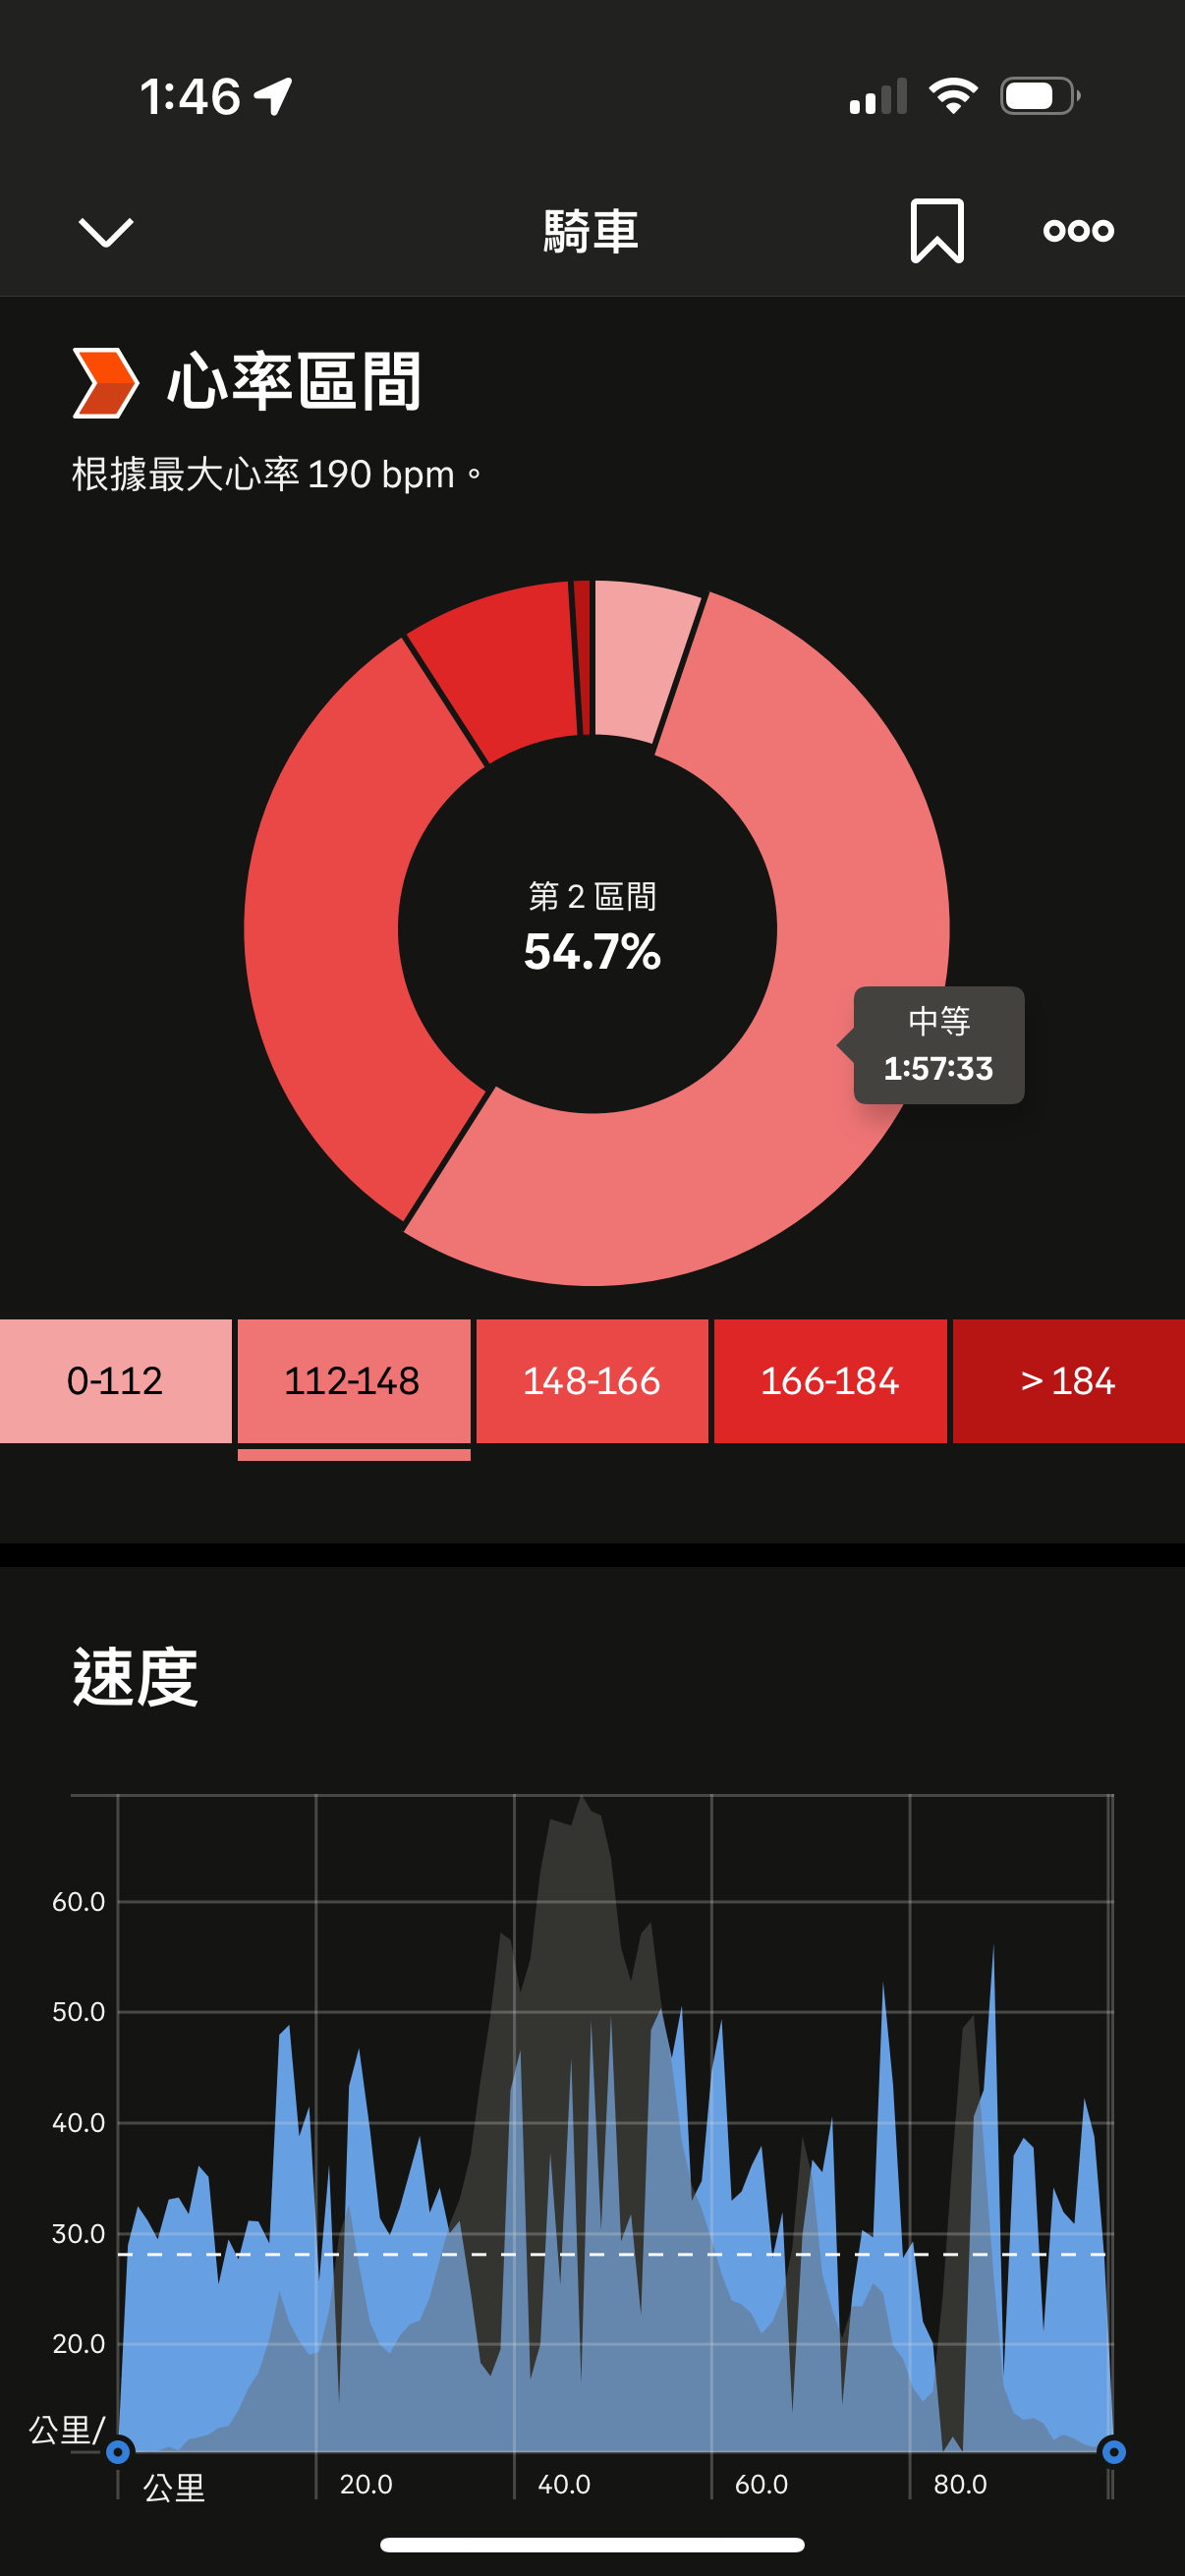
\includegraphics[height=5cm]{subscribe4.png}\pause
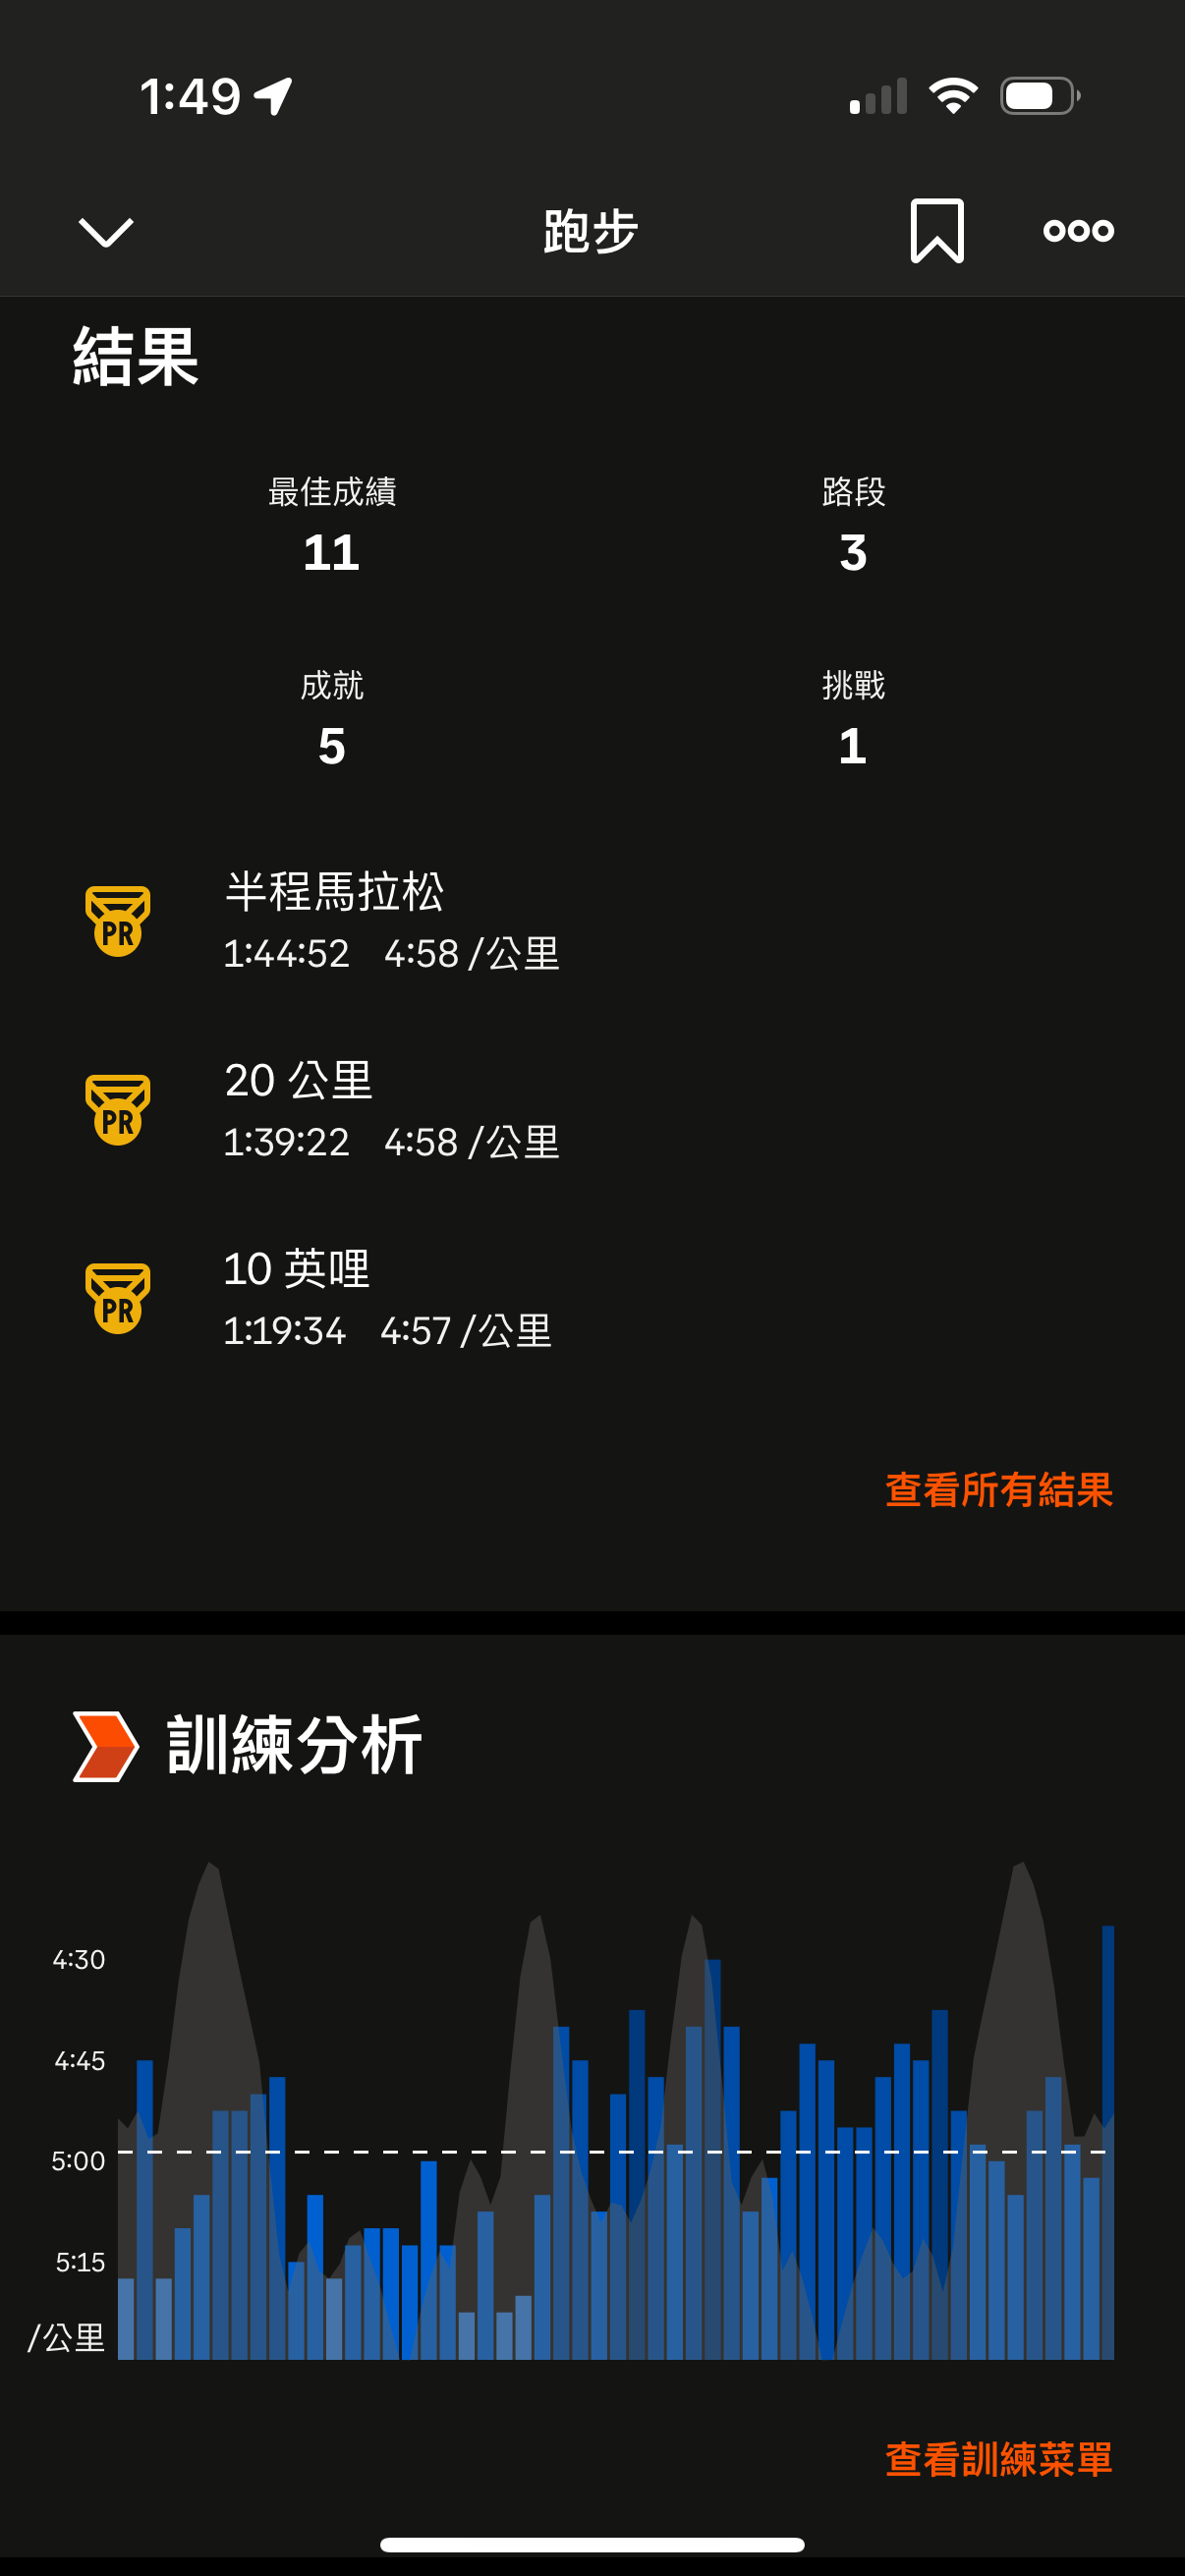
\includegraphics[height=5cm]{subscribe5.png}\pause
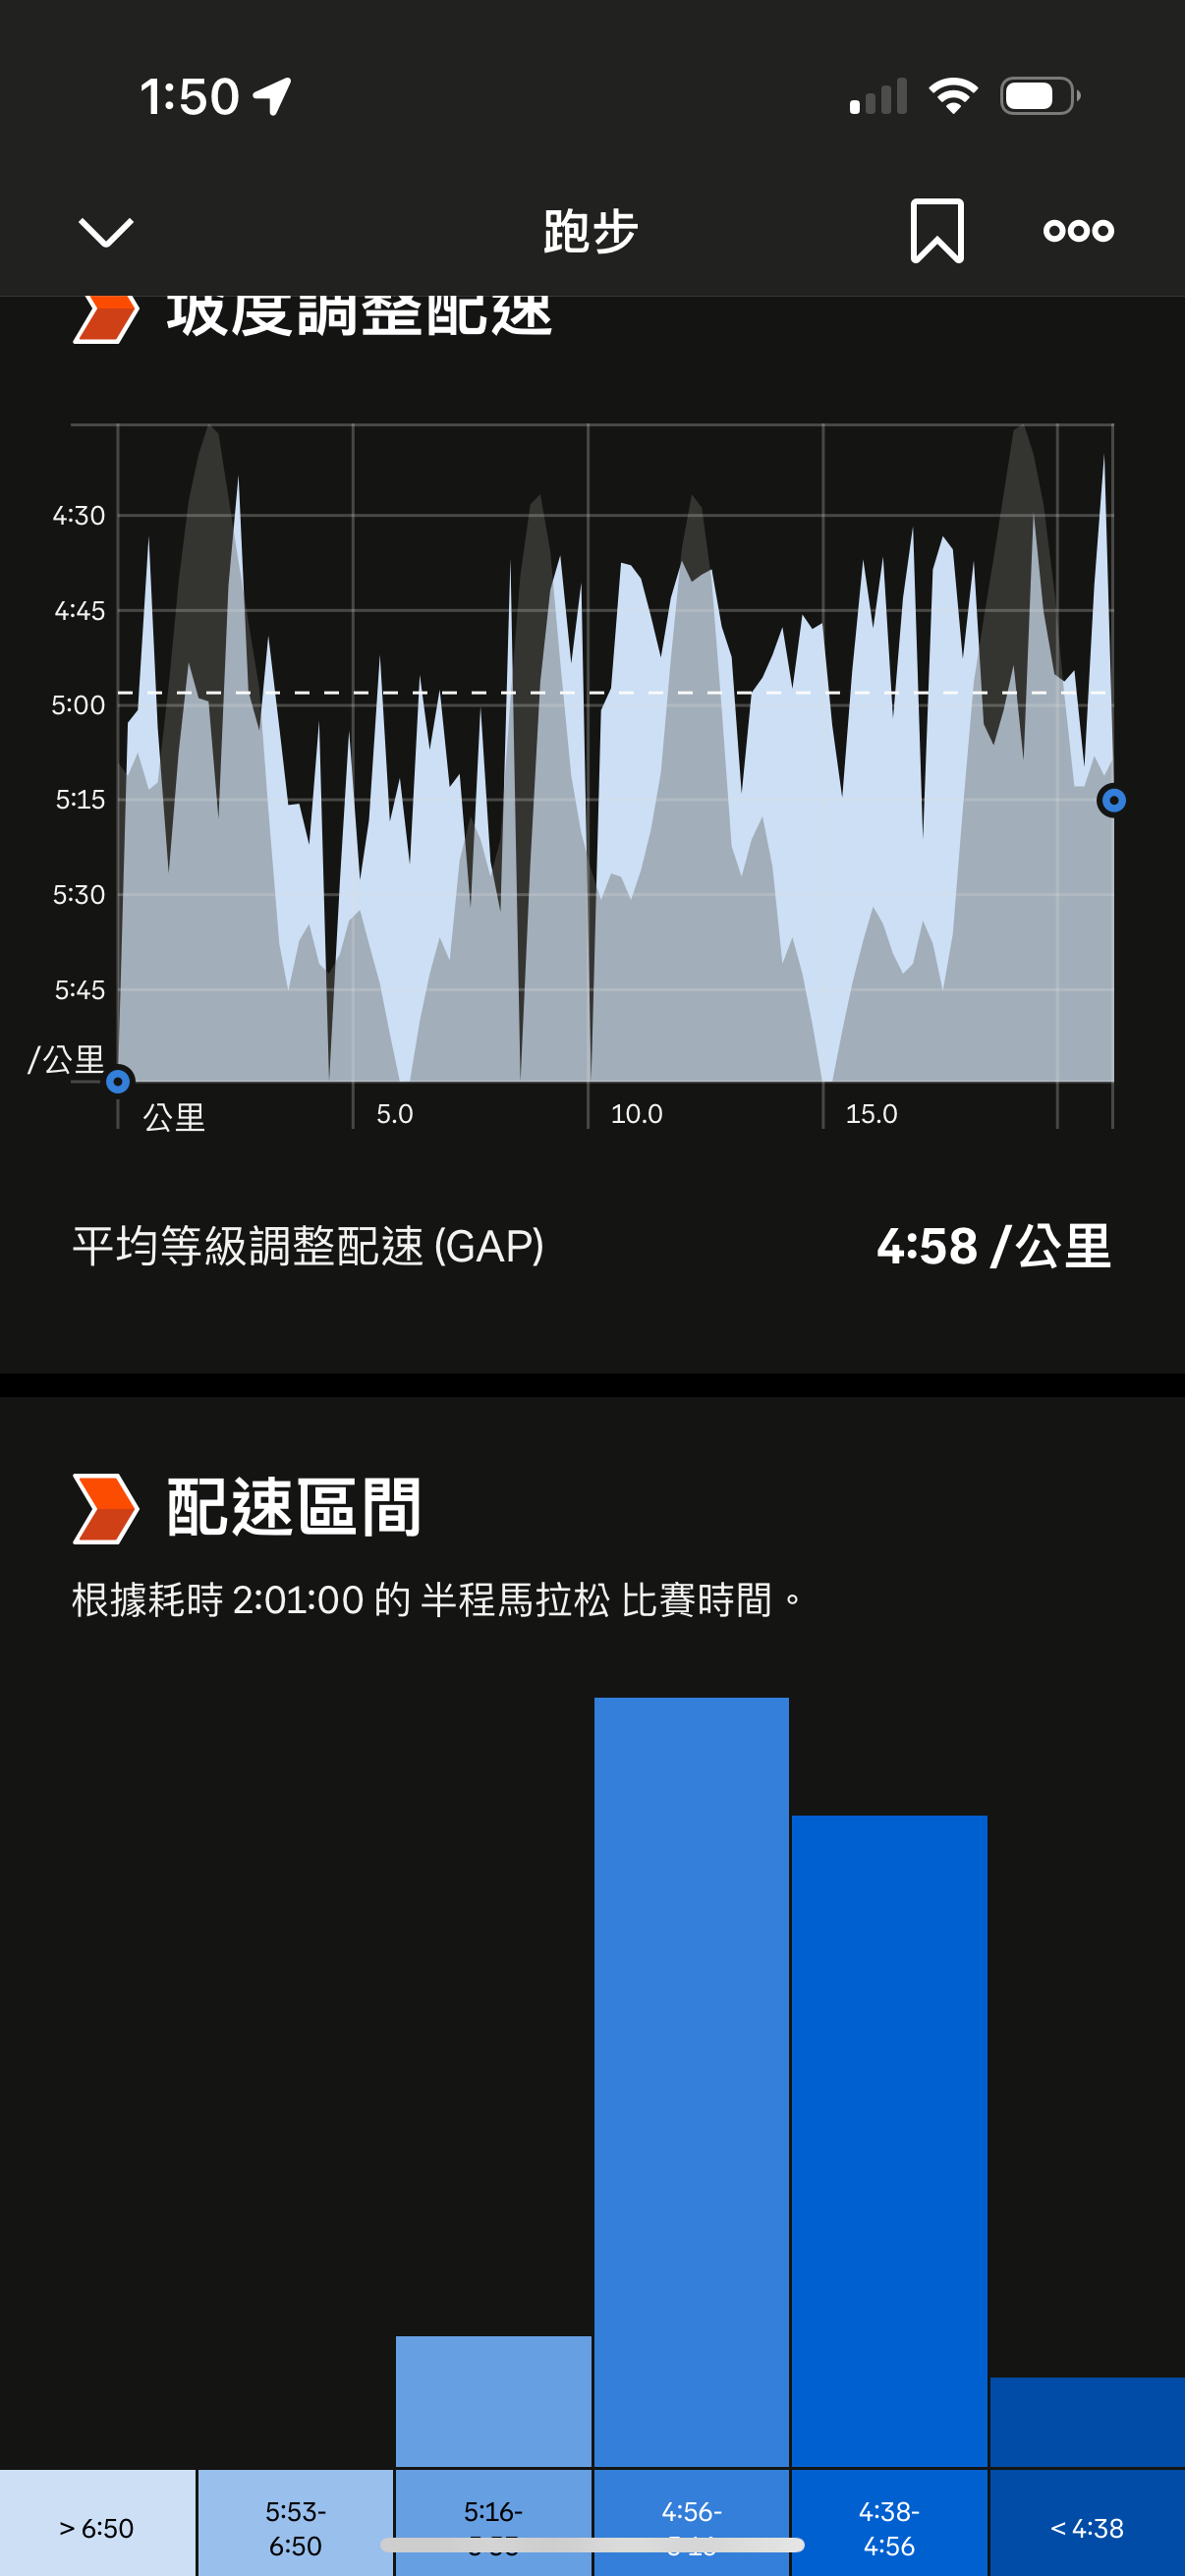
\includegraphics[height=5cm]{subscribe6.png}\pause
\item 其實只要有 GPX 檔,這些都可以自己做\pause
\item Intervals 也有類似的功能
\end{itemize}
}\only<11>{
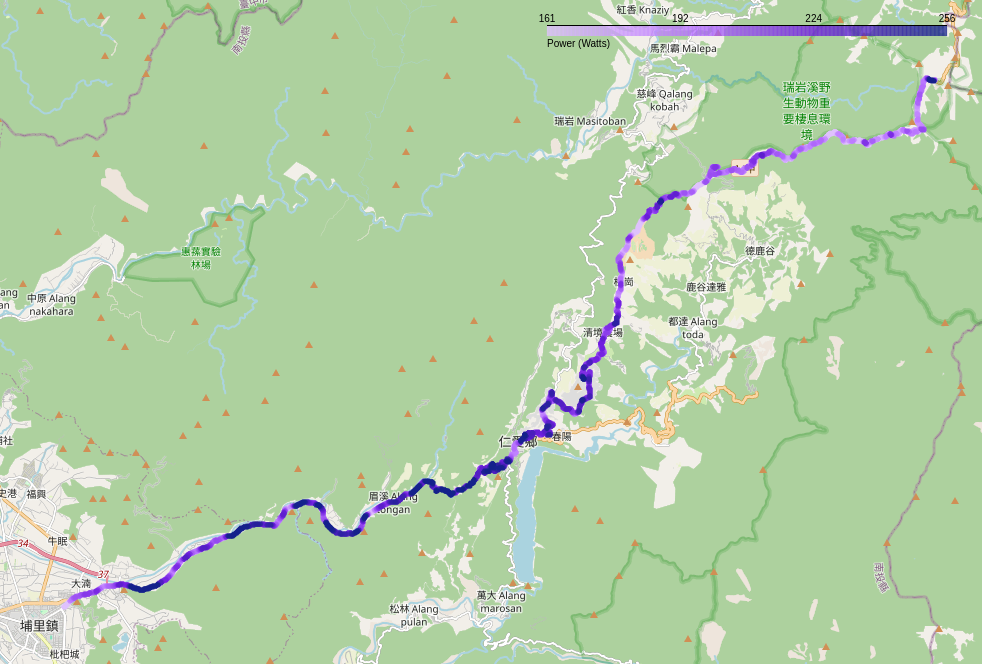
\includegraphics[height=6cm]{colorMap.png}
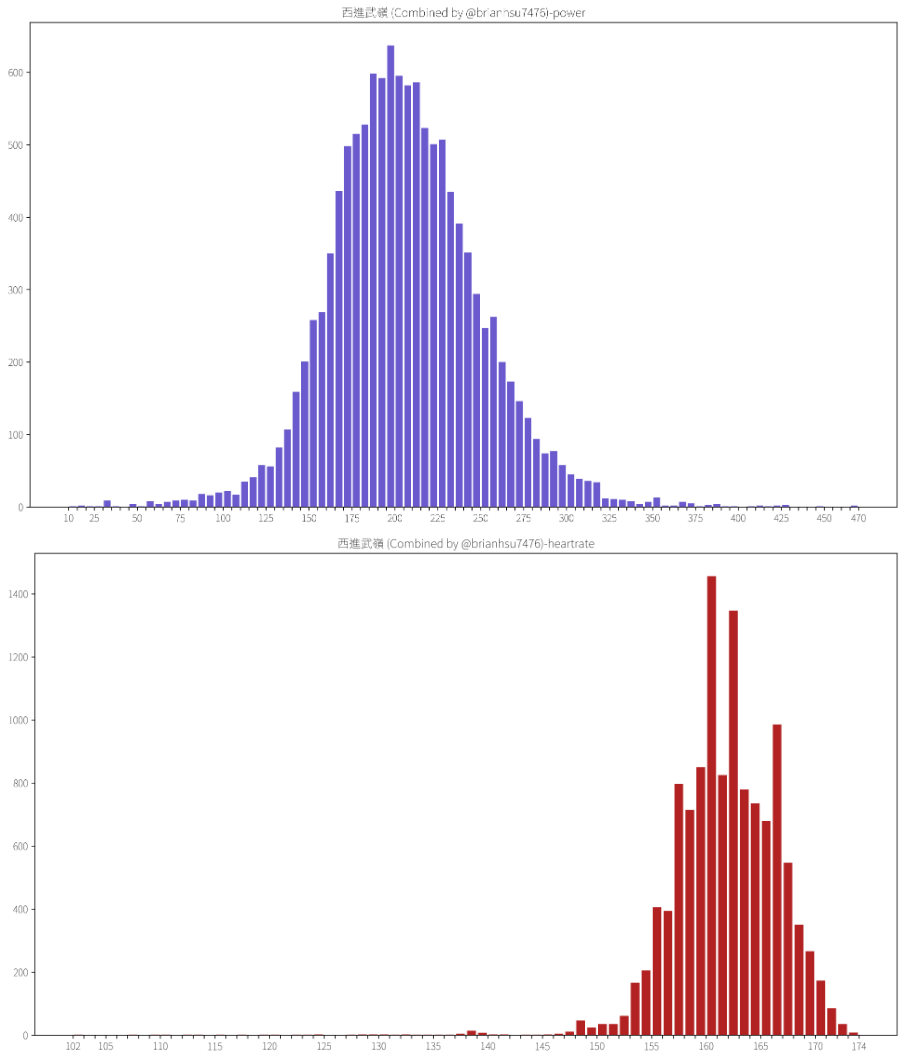
\includegraphics[height=6cm]{subscribeStats.png}
}
\end{frame}

\begin{frame}{路段排行榜}
\begin{multicols}{2}
\begin{itemize}
\item 沒訂閱只能看到男女排行榜上的前十名\pause
\item 訂閱可以看到 依年齡、體重、今天、今年、正在追蹤、社團 的排行榜,而且網頁版可以看到完整而非只有前10名的排行榜\pause
\item \href{http://ws1.csie.ntu.edu.tw:9480}{Who Is the 80 King?}:稍微完整一些的排行榜,收集了有標星號的路段,有追蹤或是有在台大單車社 Strava 社團裡的人都會出現在排行榜上\\

\includegraphics[height=3cm]{80KingQRCode.png}
\newpage
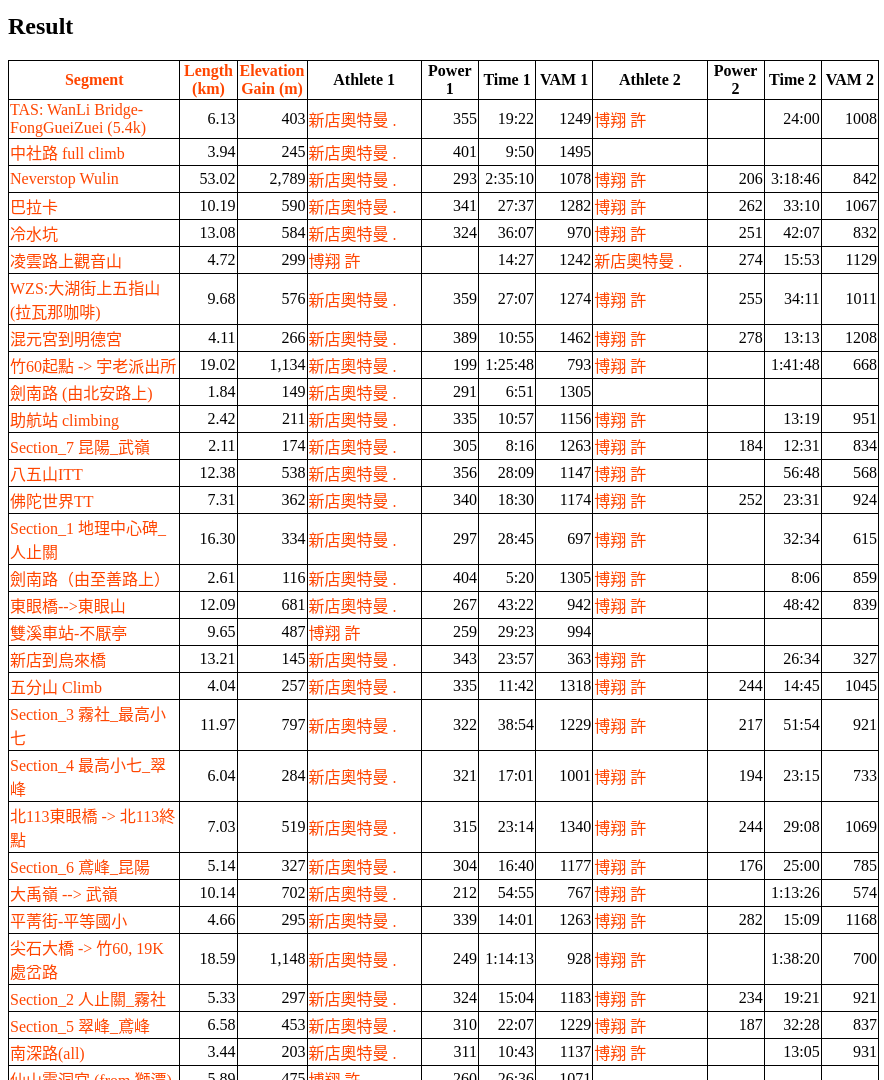
\includegraphics[height=7cm]{80King.png}
\end{itemize}
\end{multicols}
\end{frame}

\begin{frame}{路段創建(網頁版)}
\begin{itemize}
\item 當你發現某個很有趣的路段(例如118神掌,或是一條沒人探索過的山路)想與其他人競速,訂閱可以創建路段\pause
\item 創建路段的起終點不要設在太極限的位置以防計時失敗\pause
\item 盡量避免路段經過太長的山洞\\\pause
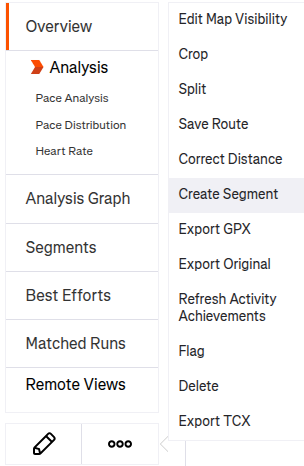
\includegraphics[height=5cm]{segmentCreate1.png}\pause
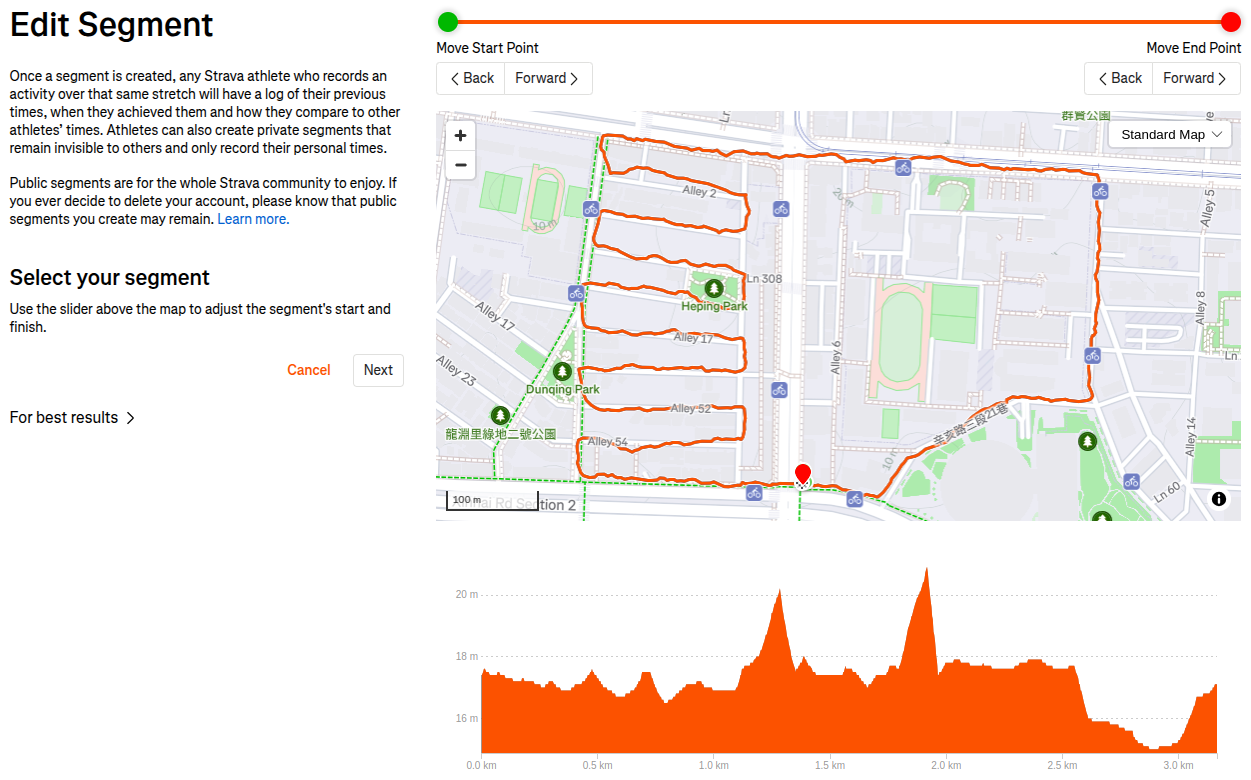
\includegraphics[height=5cm]{segmentCreate2.png}
\end{itemize}
\end{frame}

\begin{frame}{路線繪製}
\begin{itemize}
\item 訂閱可以繪製路線\pause
\item Strava 的路線會照 global heatmap 去畫,所以畫出來的路線會是車友常騎的路線\pause
\item Strava 會告訴你一條路線的路況大致上如何\\\pause
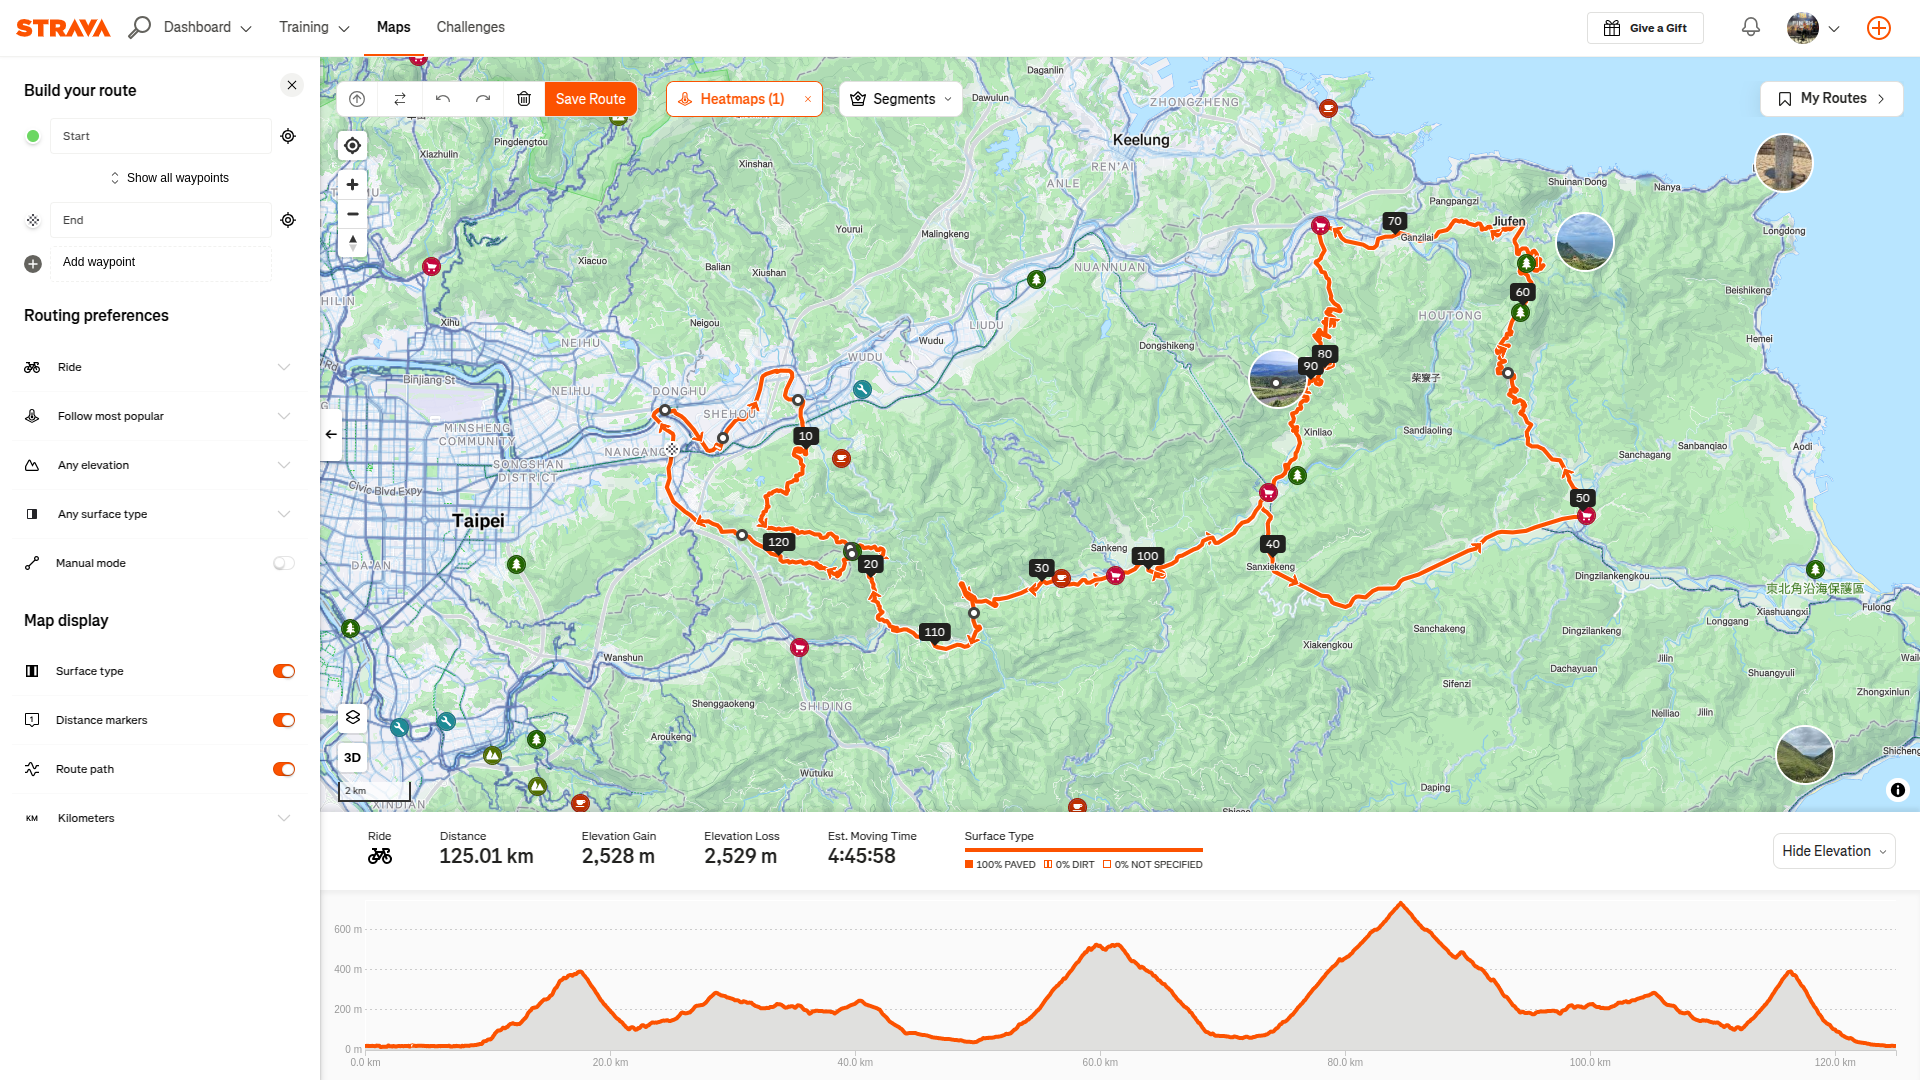
\includegraphics[height=6cm]{routeCreate.png}
\end{itemize}
\end{frame}
